\chapter{Influenza A gradual and epochal evolution: insights from  simple models}
% Insert Author names, affiliations and corresponding author email.

Sébastien Ballesteros$^{1,\ast}$, 
Elisabeta Vergu$^{2}$, 
Bernard Cazelles$^{1,3}$
\\
1 UMR 7625  (UPMC, ENS, AgroParisTech, CNRS), Ecole Normale Supérieure, Unit of Eco-Evolutionary Mathematics,  46 rue d'Ulm, F-75230 Paris Cedex 05, France.
\\
2 INRA, UR341 Mathématiques et Informatique Appliquées, F-78352 Jouy en Josas, France
\\
3 UMMISCO UMI 209 IRD-UPMC, 93142 Bondy, France
\\
$\ast$ E-mail: sebastien.ballesteros@biologie.ens.fr


% Please keep the abstract between 250 and 300 words
\section*{Abstract}

The recurrence of influenza~A epidemics has originally been explained
by a ``continuous antigenic drift'' scenario. Recently, it has been
shown that if genetic drift is gradual, the evolution of influenza A
main antigen, the haemagglutinin, is punctuated. As a consequence, it
has been suggested that influenza A dynamics at the population level
should be approximated by a serial $SIR$ model.
%%%%%%%%%%%%%%%%%
Here, simple models are used to test whether a serial $SIR$ model
requires gradual antigenic drift within groups of strains with the
same antigenic properties (antigenic clusters). We compare the effect
of status based and history based frameworks and the influence of
reduced susceptibility and infectivity assumptions on the transient
dynamics of antigenic clusters.
%%%%%%%%%%%%%%%%%
Our results reveal that the replacement of a resident antigenic
cluster by a mutant cluster, as observed in data, is reproduced only
by the status based model integrating the reduced infectivity
assumption. This combination of assumptions is useful to overcome the
otherwise extremely high model dimensionality of models incorporating
many strains, but relies on a biological hypothesis not obviously
satisfied. Our findings finally suggest the dynamical importance of
gradual antigenic drift even in the presence of punctuated immune
escape. A more regular renewal of susceptible pool than the one
implemented in a serial $SIR$ model should be part of a minimal theory
for influenza at the population level.


% Please keep the Author Summary between 150 and 200 words
% Use first person. PLoS ONE authors please skip this step. 
% Author Summary not valid for PLoS ONE submissions.   
%\section*{Author Summary}

\section{Introduction}

Currently, two subtypes of influenza type A virus (H3N2 and H1N1)
cocirculate in human populations along with the influenza type B
virus. In temperate zones and during inter-pandemic periods, their
dynamics lead to annual epidemics of variable amplitude caused by
alternating types and subtypes \citep{Nelson2007}. Worldwide, these
annual epidemics result in about three to five million cases of severe
illness, and about 250 000 to 500 000 deaths \citep{WHO2003}.

The recurrence of influenza A epidemics is still not thoroughly
understood despite a large amount of empirical and theoretical
investigations. It has originally been explained by the evolution of
the main surface glycoproteins of the virus (mainly haemagglutinin,
HA, but also Neuraminidase, NA) inducing possible “reinfection” of
previously infected hosts. This ``continuous antigenic drift''
scenario \citep{Pease1987} where viruses continuously escape immunity
as mutations accumulate has recently been challenged by new sequences
data and theoretical developments.

From the theoretical side, multi-strains models tracking the infection
history of the hosts have been difficult to use due to the exponential
growth of state variables as the number of strains increases
\citep{Andreasen1997}. Nevertheless, by using a status based approach
combined with the assumption that a previous infection reduces
infectivity and that co-infections are allowed, \citet{Gog2002} have
produced a model where the number of state variables grows linearly
with the number of strains. It has thus been possible to study how
immunologically cross-reactive strains sequentially invade a partially
susceptible population. The results of \citet{Gog2002} model, using a
linear antigenic space, have shown a self-organisation of the strains
into antigenic clusters. This organisation results in a punctuated
antigenic evolution based on a continuous genetic change, challenging
the idea of a gradual antigenic drift.

From the observational and experimental side, \citet{Smith2004} have
mapped the antigenic and genetic evolution of influenza virus from
real data using statistical techniques. They have confirmed the
theoretical results of \citet{Gog2002}, with antigenic clusters
emerging and replacing each other every 2 to 8 years.


Other theoretical works have enabled to relax the hypothesis of a
linear antigenic space \citep{Ferguson2003, Girvan2002}. Such a gain
in realism has resulted in an intuitive explosion of strains diversity
due to a positive feedback. As the antigenic diversity of
co-circulating strains increases, the production of further variants
is also increased. The key theoretical question has thus been to
explain how the strain diversity could be restricted to be compatible
with the phylogenetic tree of the glycoprotein HA of the subtype H3N2
\citep{Grenfell2004}. \citet{Ferguson2003} (see also
\citet{Andreasen2006, Minayev2008}) have included in their model a
strain transcendent temporary immunity (previously suggested by
\citet{Webster1992}), along with some sources of variability
\citep{Tria2005}. This approach allows simulating realistic viral
evolution at the sequence level. Nevertheless, it remains difficult to
prove conclusively the physiological support of this non permanent
immunity through appropriate experiments.

Recently, \citet{Koelle2006} have been able to reproduce the dynamics
of influenza HA genetic diversity within a high dimensional antigenic
space without invoking the temporary cross-immunity.
\citet{Koelle2006} model focuses on antigenic clusters resulting from
a degenerated genotype to phenotype map. The authors have considered
that the evolution of the main antigen of influenza A has two
principal characteristics: first, it consists of long periods of
stasis where antigenic clusters globally do not change their antigenic
properties but evolve through neutral or almost neutral mutations;
second, these periods are punctuated by bursts of positive selection
which precipitate antigenic cluster transitions due to rare escape
mutations. The occurrence of new antigenic clusters results in
selective sweeps that restrict strains diversity. \citet{Koelle2006}
model have shown that weak within cluster selection and the selective
sweeps that accompany antigenic clusters transition are sufficient to
recover most of HA interpandemic evolutionary dynamics, a finding
confirmed by genetic data analyses \citep{Blackburne2008, Wolf2006}.
\citet{Koelle2006} results suggest a new starting point for the
investigation of influenza dynamics at the population level. 
\vspace{1cm}

Here we are interested in the consequences of \citet{Koelle2006}
results at the population level. Contrary to the classical $SIRS$
model of \citet{Pease1987}, which resorts to a gradual antigenic
drift, \citet{Koelle2006} results suggest to focus on a serial $SIR$
model with discrete $R$ to $S$ transitions provoked by punctuated
evolution (rare immune-escape mutants with strong antigenic effects).
We are interested in contrasting the serial SIR paradigm and the
classical SIRS model of \citet{Pease1987}. In particular, we seek to
determine whether a serial $SIR$ model would require gradual antigenic
drift within clusters. As revealed by \citet{Koelle2006} study,
gradual antigenic drift favours antigenic cluster change by
facilitating the antigenic space exploration and also increases
susceptible renewal. Our approach mainly neglects the epidemiological
impact of gradual antigenic drift to disentangle the complex causal
links induced by the interactions between births and deaths processes,
gradual antigenic drift, clusters change, external virus
reintroductions and specific modelling assumptions. Our objective is
to use simple and tractable models to determine to what extent a
serial $SIR$ model per se, \textit{i.e} neglecting gradual antigenic
drift can constitute a minimal model for influenza A dynamics at the
population level.

Our analysis mainly focuses on transient dynamics that appear of first
importance for selective sweeps and antigenic clusters replacement. To
our knowledge, contrary to what has been done for the stationary
dynamics (see \citet{Dawes2002}), no study has focused on the
consequences of these modelling assumptions on the \emph{transient}
dynamics.

From the methodological side, we start by clarifying the effects of
classical modelling assumptions of multi-strains SIR models on the
invasion and persistence of a new antigenic cluster. History and
status based two-strain models including reduced infectivity and
susceptibility assumptions are considered (section Methods).
Significance and choice of biologically relevant numerical values for
model parameters are then discussed. The deterministic framework is
first explored (sections Results). Then, both stochasticity and
external reintroduction of viruses are added in order to test the
robustness of the obtained transient dynamics. Finally we discuss the
biological limitations of the only model able to reproduce observed
antigenic cluster replacement dynamics and, more generally, the
ingredients of a minimal theory for influenza A.
%
Our findings globally suggest the impact of the modelling assumptions
on the outcome of the invasion of a new antigenic cluster. They also
stress the dynamical importance of gradual antigenic drift in a
minimal theory for influenza at the population level even in the
presence of punctuated immune escape.


% You may title this section "Methods" or "Models". 
% "Models" is not a valid title for PLoS ONE authors. However, PLoS ONE
% authors may use "Analysis" 
\section{Methods}

In order to explore the behaviour of the serial $SIR$ model as a
minimal theory for influenza, we consider an adaptive dynamics
framework \citep{Dieckmann2002}. The \textit{resident} population is an
antigenic cluster of influenza strains at endemic equilibrium,
illustrating the long period of stasis described by \citet{Wolf2006}.
The immune escape mutation (as a consequence of a true mutation or a
re-assortment \citep{Du2008}) generates a new antigenic cluster called
the \textit{mutant}. We are interested in the outcome of the invasion
of the resident viral population by the mutant. This framework
illustrates the burst of positive selection proposed by
\citet{Wolf2006}.

\subsection{Different assumptions for the modelling of partial
  cross-immunity for co-circulating antigenic clusters; deterministic
  framework}

We study the outcome of immune escape mutations, by using two-strain
dynamical models applied to the resident and the mutant antigenic
clusters defined here above.

Two main modelling approaches have been used to study immunologically
cross-reactive strains: \textit{(i) history based (HB) models}
\citep{Andreasen1997} and \textit{(ii) status based (SB) models}
\citep{Gog2002a}. As stressed by \citet{Gog2002a} and
\citet{Kryazhimskiy2007}, in a \textit{HB} model, all hosts previously
infected by a strain $i$ become partially immune to a second strain
$j$. In \textit{SB} model, when a given host gets infected by a strain
$i$, the within-host immunological dynamics takes place and
``immediately'' generates the immunological status (immunised or not)
towards strain $j$ \citep{Gog2002a}.

Partial cross immunity can be modelled using two extreme hypotheses:
\textit{(i) reduced infectivity (RI)} or \textit{(ii) reduced
  susceptibility (RS)}. $SB$ models with $RI$ assumption exhibit the
attractive mathematical property of dimensional reduction without loss
of information, containing twice more equations that strains. The
tractability of this kind of models has been exploited in previous
works \citep{Gog2002, Koelle2006, Gog2008}.

To clarify the effect of these various assumptions, we provide a
comparison of both $RS$ and $RI$ cases in both $SB$ and $HB$ models.


\subsubsection{Status based model with reduced susceptibility
  \textit{(SBRS)} and co-infections}

We introduce the following notations: $R_\varnothing$ is the
proportion of hosts with no acquired immunity, $R_i$ is the proportion
of hosts who have acquired immunity to cluster~$i$ and $R_{ij}$ is the
proportion of hosts who have acquired immunity to clusters~$i$ and
$j$. Note that we include currently infected hosts ($I$) into the $R$
state variables. Partial cross-immunity is modelled by $\sigma$, which
represents the probability of being immunised against cluster $j$ when
infected by cluster $i$.

Using these notations and considering that co-infections are possible
during the infectious period and that infections with one antigenic
cluster reduce susceptibility to the other, we can derive (see for
instance \citet{Kryazhimskiy2007} or \citet{Gog2002a} )
equation~\eqref{eq:sbrsc}:

\begin{align}
\dot{R_\varnothing} & = \mu -\beta_1 R_\varnothing I^1 -\beta_2 R_\varnothing I^2 -\mu R_\varnothing  \label{eq:sbrsc}\\
\dot{R_1} & = (1-\sigma) \beta_1 R_\varnothing I^1 - \beta_2 R_1 I^2 -\mu R_1  \notag \\
\dot{R_2} & = (1-\sigma) \beta_2 R_\varnothing I^2 - \beta_1 R_2 I^1 -\mu R_2  \notag \\
\dot{R_{12}} & = \sigma \beta_1 R_\varnothing I^1 + \sigma \beta_2 R_\varnothing I^2 + \beta_2 R_1 I^2 + \beta_1 R_2 I^1 -\mu R_{12}  \notag \\
\dot{I^1} & = \beta_1 R_\varnothing I^1 + \beta_1 R_2 I^1 -\nu I^1  -\mu I^1 \notag \\
\dot{I^2} & = \beta_2 R_\varnothing I^2 + \beta_2 R_1 I^2 -\nu I^2  -\mu I^2 \notag 
\end{align}

Parameter interpretation and values are given in Table
\ref{tab:param}.


\subsubsection{Status based model with reduced infectivity
  \textit{(SBRI)} and co-infections}

In the case where infection by one antigenic cluster reduces the
infectivity of a subsequent infection by the other cluster, using the
same notation as in~\eqref{eq:sbrsc} and still allowing coinfections
during the infectious period, we obtain:


\begin{align}
\dot{R_\varnothing} & = \mu -\beta_1 R_\varnothing I^1 -\beta_2 R_\varnothing I^2 -\mu R_\varnothing \label{eq:sbric}\\
\dot{R_1} & = (1-\sigma) \beta_1 R_\varnothing I^1 - \beta_1 R_1 I^1  + (1- \sigma) \beta_1 R_1 I^1 - \beta_2 R_1 I^2  -\mu R_1 \notag \\
\dot{R_2} & = (1-\sigma) \beta_2 R_\varnothing I^2 - \beta_2 R_2 I^2 + (1 -\sigma) \beta_2 R_2 I^2 - \beta_1 R_2 I^1  -\mu R_2 \notag \\
\dot{R_{12}} & = \sigma \beta_1 R_\varnothing I^1 + \sigma \beta_2 R_\varnothing I^2 + \sigma \beta_1 R_1 I^1 + \sigma \beta_2 R_2 I^2 + \beta_2 R_1 I^2  + \beta_1 R_2 I^1 -\mu R_{12} \notag \\
\dot{I^1} & = \beta_1 R_\varnothing I^1 + \beta_1 R_2 I^1 -\nu I^1  -\mu I^1 \notag \\
\dot{I^2} & = \beta_2 R_\varnothing I^2 + \beta_2 R_1 I^2 -\nu I^2  -\mu I^2 \notag 
\end{align}

A precise derivation of~\eqref{eq:sbric} can be found in the appendix
of \citet{Kryazhimskiy2007}. This model can be further reduced to four
equations by defining $S_1$ and $S_2$ as $S_1 = R_\varnothing + R_2$
and $S_2= R_\varnothing + R_1$ respecitively. This leads to a
two-strain version of the model of \citet{Gog2002}.

\subsubsection{History based model}

In this framework, notations are changed to follow the infection
history of the hosts. Hosts can be susceptible to both clusters
(proportion $SS$), susceptible (or resistant) to one cluster and
infectious with the other one ($SI$ and $IS$, or $RI$ and $IR$
respectively), infectious with (or resistent to) both clusters ($II$
or $RR$ respectively) or susceptible to one cluster and resistant to
the other one ($SR$ and $RS$ respectively).

When first immunised by one cluster, hosts can be less infectious when
infected by the second cluster: the infectivity is modulated by the
parameter $s$ and the model is called the history based model with
reduced infectivity ($HBRI$). Hosts can also have a reduced
susceptibility towards the second cluster controlled by parameter $x$.
The model is called the history based model with reduced
susceptibility ($HBRS$).
 
This gives rise to the following equations~\eqref{eq:MODEL6}, with
$s,x \in [0,1]$.


\begin{align}
\dot{SS} & = \mu -\beta_1 SS (IS + s II + s IR) -\beta_2 SS (SI+ s II + s RI) -\mu SS  \label{eq:MODEL6}\\
\dot{IS} & = \beta_1 SS (IS+ s II + s IR) -\beta_2 x IS (SI+ s II + s RI) -\nu IS -\mu IS \notag \\
\dot{SI} & = \beta_2 SS (SI+ s II + s RI) -\beta_1 x SI (IS+ s II + s IR) -\nu SI -\mu SI \notag \\
\dot{II} & = \beta_2 x IS (SI+ s II + s RI) + \beta_1 x SI (IS+ s II + s IR) -\nu II -\nu II -\mu II \notag \\
\dot{RS} & = \nu IS -\beta_2 x RS (SI+ s II + s RI) -\mu RS \notag \\
\dot{SR} & = \nu SI -\beta_1 x SR (IS+ s II + s IR) -\mu SR \notag \\
\dot{IR} & = \nu II + \beta_1 x SR (IS+ s II + s IR) -\nu IR -\mu IR \notag \\
\dot{RI} & = \nu II + \beta_2 x RS (SI+ s II + s RI) -\nu RI -\mu RI \notag \\
\dot{RR} & = \nu IR + \nu RI -\mu RR \notag 
\end{align}

As noted by \citet{Kamo2002}, in the case of the \textit{RS}
assumption we can reduce the dimension of the system by introducing
the following state variables: $I^1 = IS+ II + IR$ ; $I^2 = SI+ II +
RI$ ; $R_\varnothing = SS$ ; $R_1 = IS + RS$ and $R_2 = SI + SR$.\\


Another assumption was used by \citet{Gupta1998}. In \citet{Gupta1998}
model, cross-protection does not affect susceptibility but reduces
transmissibility by a factor $s$. Instead of reducing the infectivity
of the hosts as for the previous $HBRI$ model
(equation~\ref{eq:MODEL6}) , \citet{Gupta1998} model assumes that
infection by a cross-reactive cluster of partially protected hosts
results in a partition of the infected hosts into a proportion $s$ of
infectious hosts and a proportion $(1-s)$ of non infectious hosts that
nevertheless become immunised to the infecting cluster. This
assumptions lead to equation~\ref{eq:MODEL7}.

\begin{align}
\dot{SS} & = \mu -\beta_1 SS (IS + II + IR) -\beta_2 SS (SI+ II + RI) -\mu SS  \label{eq:MODEL7}\\
\dot{IS} & = \beta_1 SS (IS+ II + IR) -\beta_2 IS (SI+ II + RI) -\nu IS -\mu IS \notag \\
\dot{SI} & = \beta_2 SS (SI+ II + RI) -\beta_1 SI (IS+ II + IR) -\nu SI -\mu SI \notag \\
\dot{II} & = s \beta_2 IS (SI+ II + RI) + s \beta_1 SI (IS+ II + IR) -\nu II -\nu II -\mu II \notag \\
\dot{RS} & = \nu IS -\beta_2 RS (SI+ II + RI) -\mu RS \notag \\
\dot{SR} & = \nu SI -\beta_1 SR (IS+ II + IR) -\mu SR \notag \\
\dot{IR} & = \nu II + s \beta_1 SR (IS+ II + IR) + (1-s) \beta_2 IS (SI+ II +RI) -\nu IR -\mu IR \notag \\
\dot{RI} & = \nu II + s \beta_2 RS (SI+ II + RI) + (1-s) \beta_1 SI (IS+ II + IR) -\nu RI -\mu RI \notag \\
\dot{RR} & = \nu IR + \nu RI + (1-s) \beta_1 SR (IS+ II + IR) + (1-s) \beta_2 RS (SI+ II + RI) -\mu RR \notag 
\end{align}

As originally proposed by \citet{Gupta1998} the dimension of
equation~\ref{eq:MODEL7} model can be reduced by introducing: $z_i$ the
proportion of hosts infectious or immunised by cluster $i$
(\textit{e.g} $z_1=IS+II+RS+IR+RI+RR$), $w_i$ the proportion of hosts
infectious or immunised by cross-reactive cluster with cluster $i$
including cluster $i$ itself (\textit{e.g}
$w_1=IS+SI+II+RS+SR+IR+RI+RR$) and $y_i$ the hosts infectious by
cluster $i$ (\textit{e.g} $y_1=IS+II+IR$).
%$(w_1-z_1)=SI+SR$
%$(1-z_1)=SS+SI+SR$
%$(1-w_1)=SS$
In case were the degree of protection against new infections is the
same for all related strains, \citet{Gupta1998} model contains only
three times more equation than strains. However, generalisation to
several levels of cross-protection greatly increases the
dimensionality \citep{Minayev2008, Minayev2009}. As the model in
equation~\ref{eq:MODEL7} and the $HBRI$ model of
equation~\ref{eq:MODEL6} lead to similar results, we will only
consider the latter one depicted by equation~\ref{eq:MODEL6}. Our
analyses will thus concern four models : $SBRS$, $SBRI$, $HBRS$ and
$HBRI$ all summarised in figure~\ref{fig:models}.



\begin{figure}[!htbp]
\begin{center}
  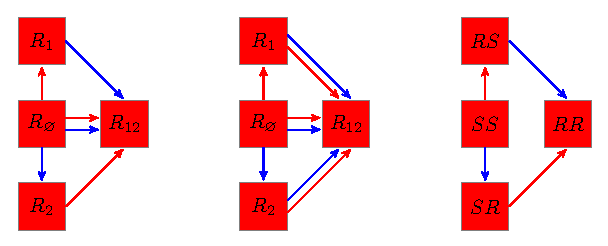
\includegraphics[width=0.8\linewidth]{graphs/article1/figure_1.eps}
\end{center}
  \caption{ $SBRS$ (left), $SBRI$ (middle) and $HB$ (both $HBRS$ and
  $HBRI$) (right) two antigenic-clusters models. Red (blue) arrows
  represent infection by antigenic cluster 1 (2). Only the $SBRI$ model
  (middle) is subject to cross-immune boosting ($R_i \to R_{ij}$
  following reinfection by strains of cluster $i$).}
\label{fig:models}
\end{figure}

\clearpage

\subsection{Stochastic models}

We implemented stochastic versions of each of these four models
($SBRS$, $SBRI$, $HBRS$ and $HBRI$) using Gillespie event-driven
algorithm \citep{Gillespie1977} and the MT19937 random number generator
of Makoto Matsumoto and Takuji Nishimura provided by the C library GSL
\citep{Galassi2003}. For instance, for the $SBRI$ model, the
differential equation system \eqref{eq:sbric} can be translated into
the reaction scheme described in Supporting Information~S1.

\subsection{Parameter values}

Two sets of parameters were used here. One consists of parameters
mainly used in theoretical papers (\textit{e.g.} \citet{Koelle2006,
  Ferguson2003, Goekaydin2007}) and the other consists of more direct
estimates of parameters from household studies (\textit{e.g.}
\citet{Cauchemez2004, Lavenu2004, Ferguson2005}). They are all defined
in Table~\ref{tab:param}. For comparison purpose, we have retained the
parameters values of \citet{Koelle2006} and have provided a
sensitivity analysis using the other set of parameters (results not
shown). Parameters $\sigma$ and $x$ (or $\sigma$ and $s$) can be
related by $x=1-\sigma$ ($s=1-\sigma$ respectively). For the sake of
simplicity, we refer to $\sigma$ only and express $x$ and $s$ with
respect to $\sigma$.


\begin{table}[!htbp]
  \caption{Parameter values}
  \begin{footnotesize}
    \begin{tabular}{|c|c|c|}
      \hline
      Parameters & Theoretical & Empirical\\
      \hline
      $\mu$ (birth and death rate) & $1/70$ years$^{-1} $ \cite{Goekaydin2007} & $1/70$ years$^{-1}$ \cite{Goekaydin2007}\\
      \hline
      $\nu$ (recovery rate) & $1/8$ days$^{-1}$ \cite{Koelle2006} & $1/2.77$ days$^{-1}$ \cite{Lavenu2004} \\
      \hline	
      $R_0$ ($\beta=R_0 (\mu+\nu)$) & $5$ \cite{Koelle2006} & $2.66$ \cite{Lavenu2004} \\
      \hline		
    \end{tabular}
  \end{footnotesize}
  \label{tab:param}
\end{table}


The choice of appropriate values for $\sigma$ was motivated by the
significance of the process captured by the model. We are mainly
interested in antigenic evolution occurring during epidemic influenza
(whether it is \textit{punctuated} or \textit{gradual}). As we work at
the phenotype level, our framework can also be used to study pandemic
influenza and \textit{antigenic shift} (appearance of new influenza
subtypes within humans). The distinction between these three processes
(gradual/punctuated antigenic drift and antigenic shift) is only based
on the value of $\sigma$ ($\sigma \in [0,1]$) taken as a bifurcation
parameters. Low $\sigma$ values ($\sigma \to 0$) are related to
\emph{antigenic shift} and $\sigma$ values close to 1 correspond to
\emph{antigenic drift}, either gradual or punctuated.
%
In order to separate punctuated from gradual antigenic drift, we use
the scale given in \citet{Koelle2006} and consider that $\sigma$
values under 0.93 are relevant for punctuated immune escape (typically
0.8), whereas higher values, closer to 1, are more appropriate for
gradual antigenic drift. Note that comparable values were used in
previous studies focusing on gradual antigenic drift \citep{Gog2002,
  Ferguson2003}

Defining the population size ($N$) is of tremendous importance when
using stochastic models \citep{Bartlett1957, Bartlett1960,
  Bartlett1964, Keeling1997a, Naasell2005}. As we are mainly
interested in replacement dynamics, we need to define a population
size where the resident cluster can persist when alone in order to
avoid confusion between different causes of replacement. According to
our simulations (Supporting Information~S1), we choose a population size of 10 million
of individuals to ensure that resident extinctions are not due to
endemic fadeout during the timescale considered (10 years,
figure~\ref{fig:deter}). This value is also used in the deterministic
framework to fix a threshold (equal to $\frac{1}{N}$) below which we
consider that extinctions occur. Note that this Critical Community
Size (CCS) \citep{Lloyd-Smith2005} does not guarantee that the
resident strain could have invaded the population and persist
\citep{Conlan2007}.


% Results and Discussion can be combined.
\section{Results}

\subsection{Invasion condition of the mutant cluster}

We start our analysis by examining the dynamical impact of the four
modelling assumptions ($SBRS$, $SBRI$, $HBRS$ and $HBRI$)
corresponding respectively to equations
\eqref{eq:sbrsc},~\eqref{eq:sbric} and ~\eqref{eq:MODEL6}) thorough
calculation of invasion conditions of the mutant cluster (labelled
cluster 2) within the environment corresponding to the equilibrium of
the resident cluster (labelled cluster 1).

For the $SB$ models, in both $SBRI$ and $SBRS$ versions, the invasion
condition can be deduced from:
\begin{align}
  \left. \frac{d I^2}{d t} \right|_{R_\varnothing^*, R_1^*} & =
  (\beta_2 R_\varnothing^* + \beta_2 R_1^* -\nu -\mu)
  I^2, \label{eq:INVASION1}
\end{align}
where $R_\varnothing^*$ and $R_1^*$ are equilibrium values of
$R_\varnothing$ and $R_1$ when only cluster 1 is present. In both
$SBRI$ and $SBRS$ models, $R_\varnothing^* = \frac{\mu +
  \nu}{\beta_1}$. For $R_1^*$, in the $SBRS$ model $R_1^{*rs} = (1 -
\sigma) \left(1 - \frac{\mu + \nu}{\beta_1} \right)$ and $R_1^{*ri} =
\frac{(1 - \sigma) \left(1 - \frac{\mu + \nu}{\beta_1} \right)}{\sigma
  \left( \frac{\beta_1}{\mu + \nu} -1 \right) +1}$ in the $SBRI$
model, that is $R_1^{*ri} = \frac{R_1^{*rs}}{\sigma \left(
    \frac{\beta_1}{\mu + \nu} -1 \right) +1} $. If parameters are
equal for the two antigenic clusters (that is
$\beta_1=\beta_2=\beta$), equation~\eqref{eq:INVASION1} becomes:
$$\left. \frac{d I^2}{d t} \right|_{R_\varnothing^*, R_1^{*}}  = \beta R_1^{*} I^2 $$
The mutant can invade (\textit{i.e.} $\left. \frac{d I^2}{d t}
\right|_{R_\varnothing^*, R_1^*} > 0$) as long as $\sigma < 1$
provided that $R_0~=~\frac{\beta}{\mu + \nu}~>~1$. The invasion
fitness of the $SBRI$ model equals the one of the $SBRS$ model divided
by $\sigma \left( \frac{\beta}{\mu + \nu} -1 \right) +1$. Depending on
$\sigma$, the initial speed of invasion with the \textit{RI}
assumption can be greatly decreased. \textit{RS} and \textit{RI}
assumptions are not without effects on the transient dynamics of
antigenic clusters invasion in SB models.

In the \textit{HB} framework, the previous approach is not feasible
for the $HBRI$ model. The basic reproduction ratio $R_0$ is 
calculated in this case as the dominant eigenvalue of the linear next generation
operator \citep{Diekmann2000}.  In both $HBRS$ and $HBRI$ models the
dominant eigenvalue is:
$$R_0^{inv} = \frac{\beta_2 SS^* + \beta_2 s x RS^* +\beta_2 s x IS^*}{\mu+\nu}$$.
As for the \textit{SB} cases, $SS^*$, $IS^*$ and $RS^*$ are
equilibrium values of $SS$, $IS$ and $RS$ when only cluster 1 is
present and are equal to $SS^* = \frac{\mu + \nu}{\beta_1}$, $IS^* =
\frac{\mu}{\mu + \nu} - \frac{\mu}{\beta_1}$ and $RS^* =
\frac{\nu}{\mu + \nu} - \frac{\nu}{\beta_1}$. If $\beta_1 = \beta_2$,
the invasion is possible (\textit{i.e.} $R_0^{inv} >1$) as long as $s
x > 0$ provided $R_0~=~\frac{\beta}{\mu + \nu}~>~1$. Contrary to the
\textit{SB} framework, in a two-cluster \textit{HB} model, invasion
fitness is the same in both \textit{RS} and \textit{RI} cases.

Table \ref{tab:R0} provides a comparison of the $R_0^{inv}$ for the
four models considered and reveals that the $SBRI$ model differs from
the three others which possess the same $R_0^{inv}$.  The $SBRI$ model
assumption appears to reduce the initial speed of invasion of the
mutant cluster by a factor $\frac{1}{\sigma (R_0 -1) +1}$.


\begin{table}[!ht]
  \caption{Invasion $R_0$}
  \begin{tabular}{|c|c|}
    \hline
    model & $R_0^{inv}$ \\
    \hline
    $SBRI$ & $1 + (1-\sigma)(R_0 -1)/(\sigma (R_0-1) +1)$ \\
    \hline
    $SBRS$ & $1 + (1-\sigma)(R_0 -1)$\\
    \hline
    $HBRI$ & $1 + sx (R_0 -1)$\\
    \hline
    $HBRS$ & $1 + sx (R_0 -1)$\\
    \hline
  \end{tabular}
  \begin{flushleft} Comparison between the four two-cluster models (equations
    \eqref{eq:sbrsc}, ~\eqref{eq:sbric} and ~\eqref{eq:MODEL6}) in terms
    of the basic reproduction ratio ($R_0^{inv}$) of the mutant cluster
    invading a resident population at endemic equilibrium.
  \end{flushleft}
  \label{tab:R0}
\end{table}



\subsection{Invasion and extinction}

\subsubsection{Deterministic framework}

Figures~\ref{fig:deter}, \ref{fig:deter_rescaled} and Supporting
Information~S1, illustrate a comparison of the effect of $\sigma$ on
the invasion dynamics of a new cluster (the resident being at endemic
equilibrium) for the four two-cluster models studied with parameters
set at theoretical values (Table \ref{tab:param}). Figure
\ref{fig:reinv_theo12} summarises the results of the transient
dynamics of the mutant invasion in terms of clusters replacement
considering a deterministic threshold of $\frac{1}{N}=10^{-7}$ for
extinction as determined by simulations summarized in Supporting
Information~S1.


\begin{figure}[!htbp]
\begin{center}
	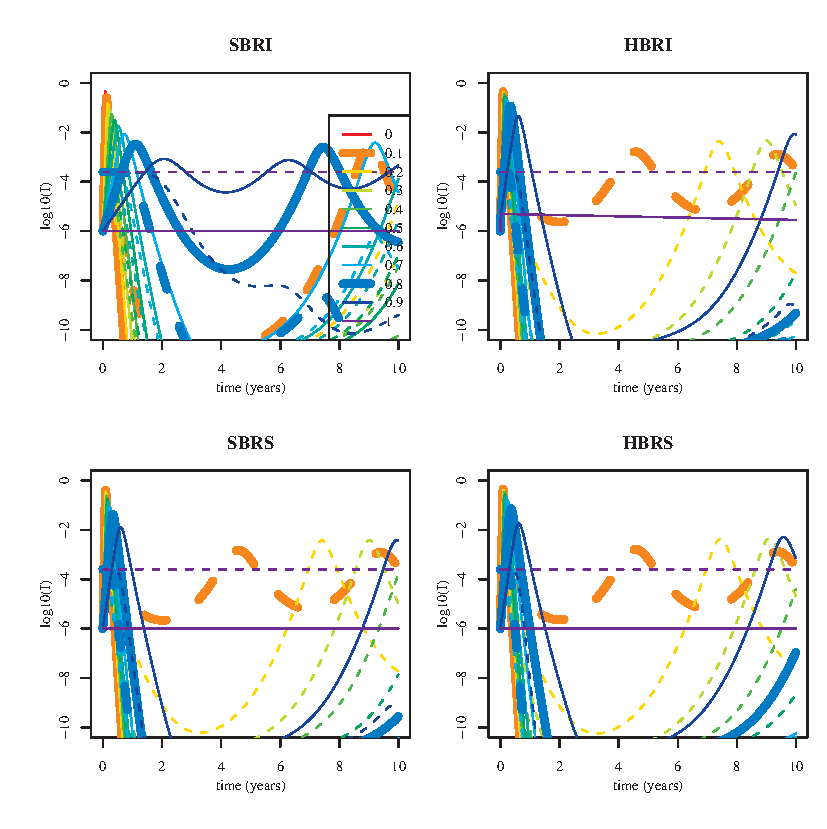
\includegraphics[]{graphs/article1/figure_2.eps}
\end{center}
        \caption{ Transient invasion dynamics for the four two-cluster
          models studied. The decimal logarithm of the proportion of
          infectious hosts for the mutant antigenic cluster (plain
          lines) and for the resident cluster (dashed lines) is
          represented as a function of $\sigma$. Colours correspond to
          different partial cross-immunity ($\sigma$) values: from
          $\sigma=0$ (antigenic shift, no cross-immunity) to
          $\sigma=1$ (antigenic drift, full cross-immunity). Parameter
          values are given in Table \ref{tab:param} (theoretical set).
          Initial conditions are : ${I^1}(0) = {I^1}^*=250.4*10^{-6}$,
          ${I^2}(0)=10^{-6}$.}
\label{fig:deter}
\end{figure}



\begin{figure}[!htbp]
\begin{center}
	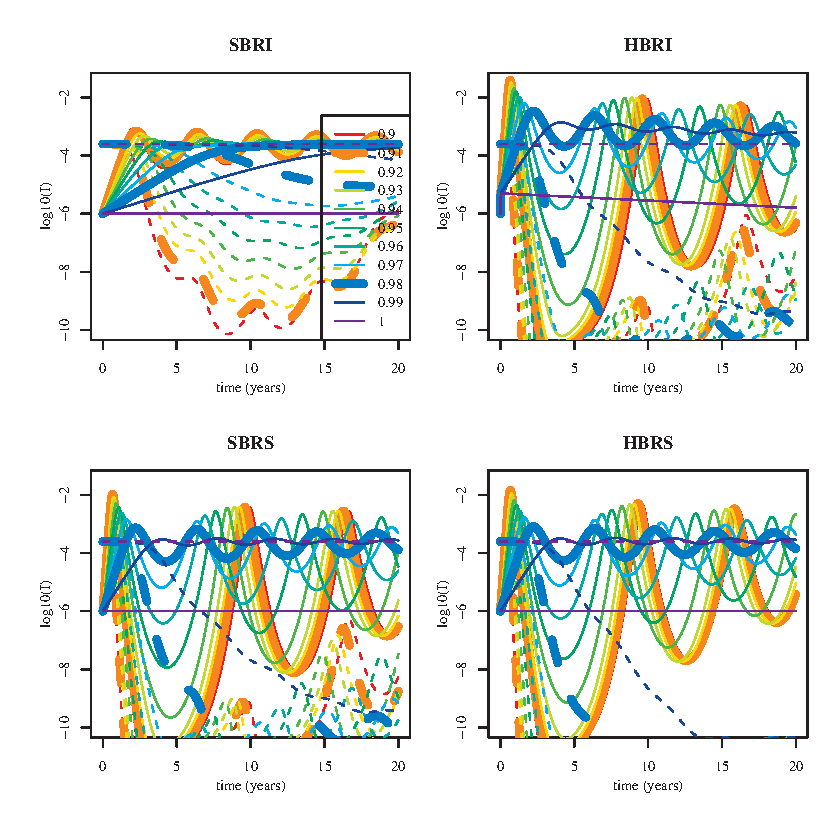
\includegraphics[]{graphs/article1/figure_3.eps}
\end{center}
        \caption{ Detail of figure~\ref{fig:deter}. Partial
          cross-immunity ($\sigma$) values more relevant for gradual
          antigenic drift ($\sigma \in [0.9,1]$).}
	\label{fig:deter_rescaled}
\end{figure}



\begin{figure}[!htbp]
\begin{center}
	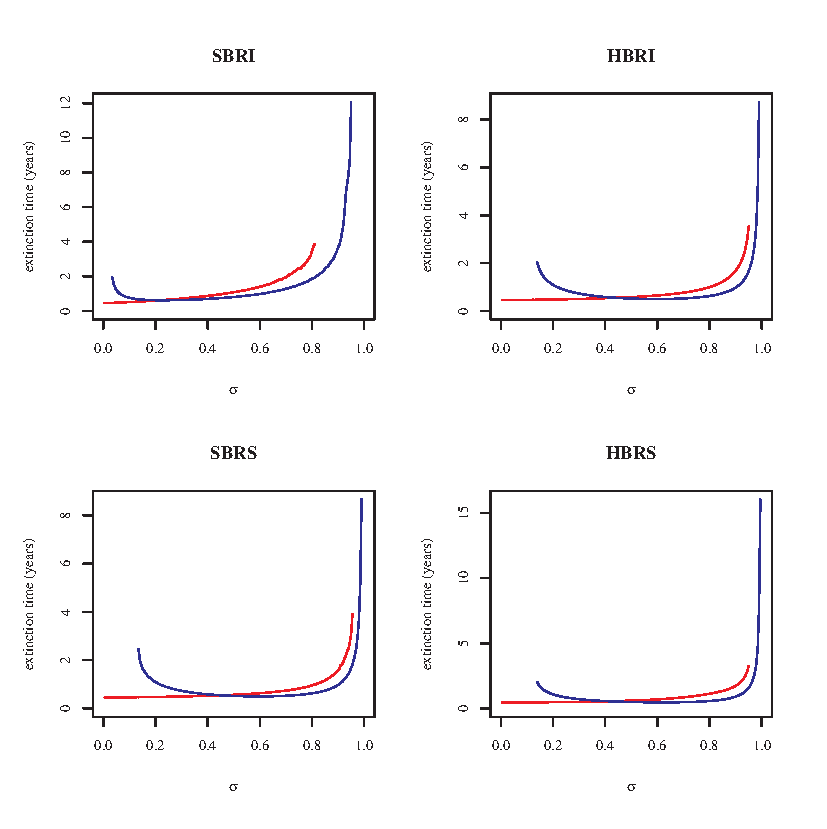
\includegraphics[]{graphs/article1/figure_4.eps}
\end{center}
\caption{ Extinction times of the resident
  antigenic cluster (blue) and of the mutant cluster (red) for the
  four two-cluster models studied. Parameter values are given in Table
  \ref{tab:param} (theoretical set). Initial conditions are :
  ${I^1}(0) = {I^1}^*=250.4*10^{-6}$, ${I^2}(0)=10^{-6}$.}
\label{fig:reinv_theo12}
\end{figure}


For $\sigma \in [0.8, 0.93[$ (corresponding to \citet{Koelle2006}
scale of rare immune escape mutations) in figures~\ref{fig:deter} and
\ref{fig:reinv_theo12} antigenic cluster replacements are possible
only for the $SBRI$ model. The three other models exhibit extinction
of both antigenic clusters.
%
For $\sigma \to 1$ (corresponding to gradual antigenic drift) in
figures~\ref{fig:deter_rescaled} and \ref{fig:reinv_theo12} the $SBRI$
model results in coexistence of both clusters contrary to the three
other models which predict the replacement.
%
For $\sigma \to 0$ (antigenic shifts) in figure~\ref{fig:deter} and
\ref{fig:reinv_theo12} the resident influenza subtype is not
sufficiently affected by the mutant subtype to go extinct and it
survives while the mutant disappears after generating an outbreak.
Note that smaller values of cross-immunity are sufficient for the
$SBRI$ model to drive the resident to extinction
(figures~\ref{fig:deter} and \ref{fig:reinv_theo12}).

In all cases, a proper rescaling of the $SBRI$ model with lower
$\sigma$ values as suggested in Table~\ref{tab:R0} is needed to render
it comparable to the three others models.

\clearpage

\subsubsection{Stochastic  framework}

Simulated trajectories corroborate the trends provided by
deterministic models, especially the particularity of the $SBRI$ model
(figures~\ref{fig:replace}, and Supporting Information~S1).



\begin{figure}[!htbp]
\begin{center}
	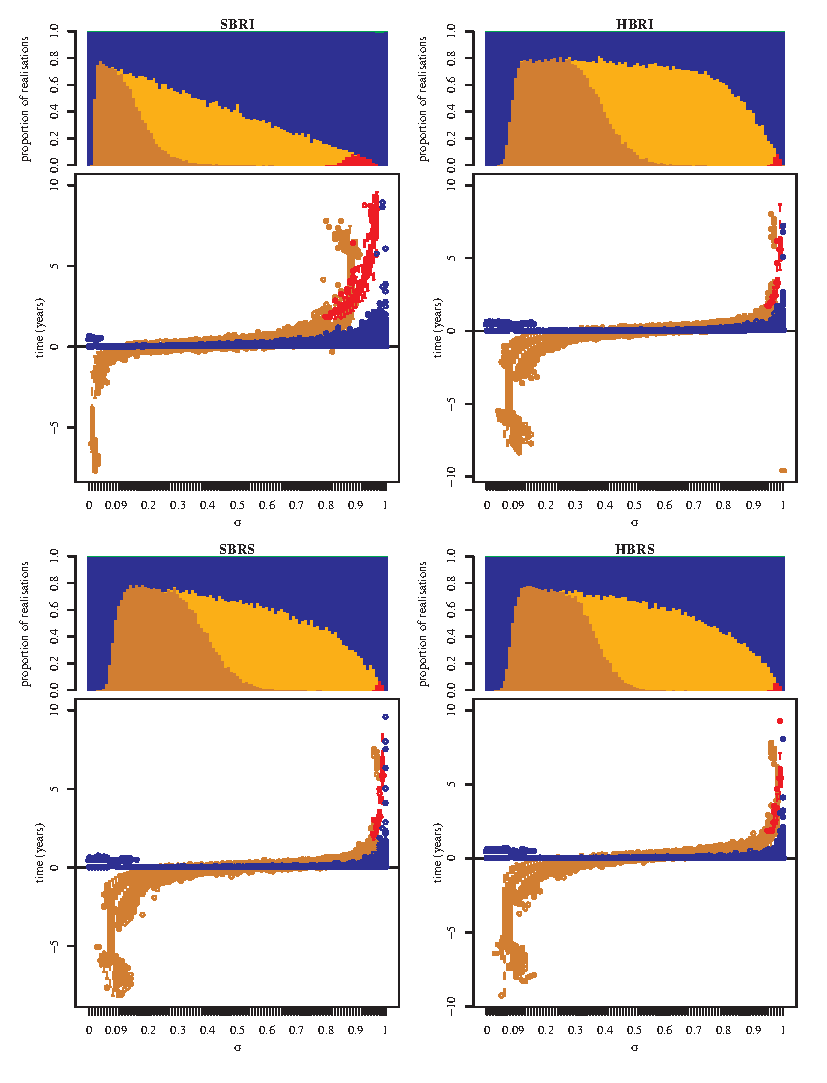
\includegraphics[width= 0.85 \linewidth]{graphs/article1/figure_5.eps}
\end{center}
        \caption{ Outcomes of the transient invasion dynamics based on
          1000 realisations of the four two-cluster stochastic
          models. For each panel, top graphs represent the proportion
          of realisations where, after 10 years: both antigenic
          clusters go extinct, but the mutant goes extinct first
          (brown); both antigenic clusters go extinct, but the
          resident goes extinct first (aborted replacement, orange);
          the resident cluster only goes extinct (successful
          replacement, red); the mutant cluster only goes extinct
          (blue); no cluster goes extinct (coexistence, green). For
          each panel, bottom box plots represent: extinction times of
          the mutant cluster when only this cluster goes extinct
          (blue); extinction times of the resident cluster when only
          this cluster goes extinct (red); the differences between
          extinction times of the mutant cluster and the resident when
          both clusters go extinct (brown and orange). Initial
          conditions: one infected individual with the mutant
          antigenic cluster is introduced in a population where the
          resident cluster is at the deterministic endemic
          equilibrium. The remaining initial conditions are those
          corresponding to the endemic equilibrium of the
          deterministic model and parameter values are given in
          Table~\ref{tab:param} (theoretical set).}
\label{fig:replace}
\end{figure}



The replacement of antigenic clusters following rare mutations with
strong antigenic effect appears to be realistic only in the case of
the $SBRI$ model (figure~\ref{fig:replace}, red bars and Supporting
Information~S1) for which a set of $\sigma$ values consistent with
punctuated immune escape variability exists. For these $\sigma$ values
($\sigma \in [0.8,1[$), a trade-off exists between invasion ability
(that is risks of initial extinction) and risk of epidemic fade-outs
(as described for the evolution of the recovery rate by
\citet{Keeling2000}).  Figure~\ref{fig:replace} shows that the
proportion of initial extinctions, previous to an epidemic caused by
the mutant, decreases as long as the degree of immune escape
($1-\sigma$) increases (blue colour in panel $SBRI$ of
figure~\ref{fig:replace}). At the same time, the proportion of
epidemic fade-outs after replacement increases (orange colour in panel
$SBRI$ of figure~\ref{fig:replace}). Moreover, these results are
consistent with formulas given in Table \ref{tab:R0}, since the
probability of initial extinctions of the mutant cluster is given by
$1/R_0^{inv}$ \citep{Diekmann2000}. For the $SBRI$ model, this
probability increases linearly with $\sigma$ (figure \ref{fig:replace}
$SBRI$, blue bars) whereas for the three other models (panel $SBRI$,
$HBRI$ and $HBRS$ of figure \ref{fig:replace}, blue bars), it remains
uniformly lower and increases as $\frac{1}{R_0+(1-\sigma) (1-R_0)}$
with $\sigma$.

The time necessary to drive the resident cluster to extinction is also
a decreasing function of the immune escape intensity (red boxplot in
panel $SBRI$ of figure~\ref{fig:replace}). For $\sigma \to 1$, transient
coexistence (5 years) of both antigenic clusters is expected before
definitive replacement.

Taken together, the previous results reveal that: \textit{(i)}
antigenic clusters replacement within a serial $SIR$ model is possible
only in the case of a $SBRI$ model; \textit{(ii)} antigenic shift
results in the extinction of both subtypes (brown colour
figure~\ref{fig:replace}, trajectories in Supporting Information~S1)
or of the mutant only (blue colour figure~\ref{fig:replace}).

\subsection{External re-introductions}

\subsubsection{Modelling re-introduction}

In the real world, populations are opened to migration and extinct
clusters can be re-introduced. To complement our results we need to
evaluate the timescales of re-invasion. In particular, we focus on:
\textit{(i)} the robustness of the replacement (i.e. is the resident
able to re-establish in the population due to spatial effects of
re-introduction?); \textit{(ii)} which cluster re-invades first when
both are extinct quasi simultaneously.

Except for initial extinctions, the observed extinctions are mostly
due to deterministic forces of susceptibles depletion and not to
random fluctuations of trajectories evolving close to one individual
(low variances in the box plots of figure \ref{fig:replace}).
Incidentally, the opportunity of a second epidemic after an epidemic
fadeout for the mutant cluster or, the opportunity of re-invasion of
the resident cluster after having been extinct due to the invasion of
the mutant cluster are mostly governed by the deterministic dynamics
of susceptibles renewal \citep{Olinky2008}.

We will thus use deterministic models to compute the average time
necessary before a recurrent epidemic. A simple way to do this is to
consider a constant amount of infectious individuals entering the
population studied. Classically (\textit{e.g.} \citet{Bjornstad2002,
  Keeling2002}) the following scheme has been used:
$$\dot{I_i}=\beta(t) S_i (I_i + m p_i) + ... ,$$
where $m$ is the number of infected individuals imported from outside
(generally $m \sim N^{-1}$) and $p_i$ is the proportion of these
immigrating hosts infected with strain $i$. Note that we do not
consider infecteds from outer regions in the bookkeeping of $I_i$.

From Supporting Information~S1 we can see that the overall pattern
of transient dynamics is not affected by the modelling of external
re-introductions.

\subsection{Re-invasion time-scales}

Figure~\ref{fig:time} reveals that for $\sigma$ values relevant for
punctuated antigenic drift ($\sigma \to 1$), successful replacements
are robust to the re-introduction of the resident antigenic cluster
(\textit{i.e} the re-introduction of the resident cluster does not
lead to an epidemic). In the case of replacements where both clusters
go extinct (the resident being extinct before the mutant) the mutant
cluster re-invades first. This underlines the fact that we face a
replacement. The time until the next epidemic is nevertheless
unrealistically high ($>5$ years) to be consistent with observed
patterns of influenza yearly recurrence in the absence of antigenic
cluster changes.


\begin{figure}[!htbp]
\begin{center}
	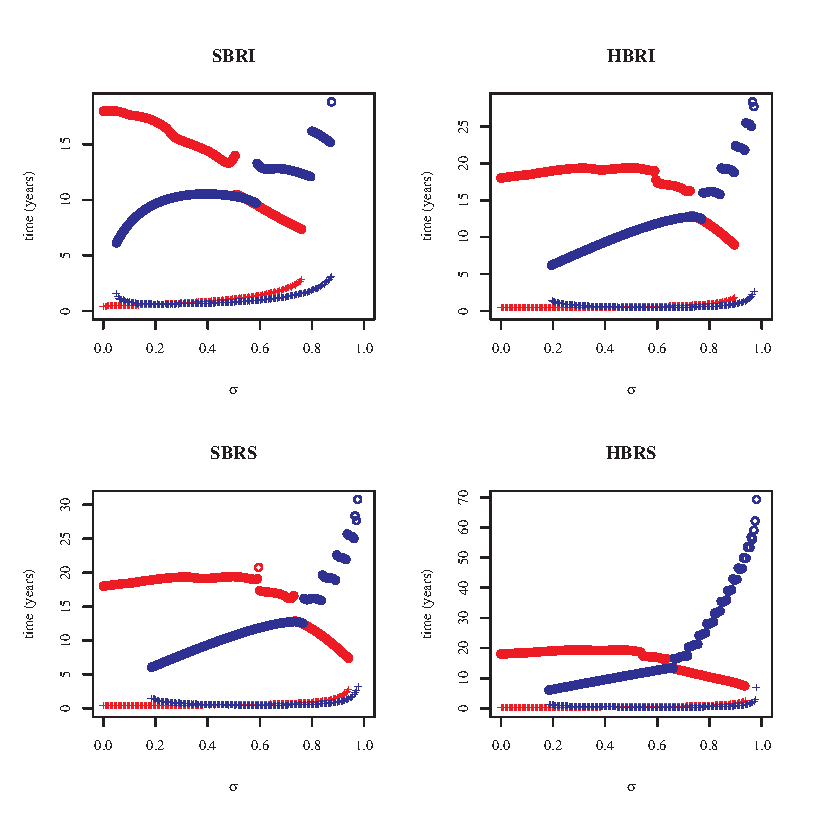
\includegraphics[]{graphs/article1/figure_6.eps}
\end{center}
	\caption{ Extinction and re-invasion times for the four
          two-cluster models in the presence of external
          reintroductions of infectious hosts. (+) represent times
          when a deterministic threshold (equal to $10^{-7}$) for
          extinction is crossed by the trajectories for the resident
          cluster (blue) and the mutant (red) ; (o) correspond to
          times of the first peak after extinction for the resident
          cluster (blue) and times of the second peak of the mutant
          cluster (red). Parameter values are given in Table
          \ref{tab:param} (theoretical set), $mp_i=10^{-8}$. Initial
          conditions are : ${I^1}(0) = {I^1}^*=250.4*10^{-6}$,
          ${I^2}(0)=10^{-6}$}
\label{fig:time}
\end{figure}


For antigenic shifts ($\sigma \to 0$), when both clusters go extinct,
timescales for a recurrent epidemic are also too long to be relevant
(re-invasion time $>10$ years, figure~\ref{fig:time}). In the case
where the invader is able to drive the resident to extinction (that is
for the $SBRI$ model), replacements are not robust to external
re-introduction. The former resident re-appears more than 10 years
before the invader.

\clearpage


\section{Discussion}

Punctuated antigenic evolution is being recognised as an important
mechanism of immune escape in various RNA viruses, but its detection
remains difficult and somewhat uncertain \citep{Cobey2008}. In this
paper we have focused on exploring to what extent the complex
processes shaping influenza dynamics can be approximated by a minimal
serial $SIR$ system, emphasising rare mutations with strong antigenic
effects. According to our results (figure~\ref{fig:deter},
\ref{fig:deter_rescaled}), punctuated immune escape results in a high
depletion of susceptibles in $SBRS$, $HBRS$ and $HBRI$ models. As a
consequence, recurrent epidemics during consecutive years are rendered
impossible even with reintroductions. However, data clearly suggest
that several recurrent epidemics of the same new mutant cluster can
follow the replacement of the resident cluster by the new one. For
instance, following its invasion, Beijing/1993 (BE93) cluster has
provoked epidemics of 1992-1993, 1993-1994, 1994-1995 and 1995-1996
seasons in New York state before being replaced by Wuhan/1995
(WU95)-like viruses \citep{Rambaut2008}. Such dynamics can only be
reproduced by the \textit{SBRI} model because it produces
comparatively slower invasion dynamics and fewer susceptible
depletion. A minimal serial \textit{SIR} theory is thus supported only
within the $SBRI$ framework.

In the following, we review the processes that makes the $SBRI$ model
different from \textit{HB} or \textit{SB} models with \textit{RI}
assumption. We then provide elements pointing out that these processes
direct towards a biologically problematic description of
cross-immunity. Finally, we provide arguments supporting the idea
already evoked by \citet{Koelle2006} that a sequential $SIR$ model
requires within antigenic cluster gradual antigenic drift and that
this process should be part of a minimal theory for influenza dynamics
at the population level.

\subsection{Is the $SBRI$ model particularly appropriate?}

One of the important aspects of influenza dynamics is the
cross-immunity represented here by the parameter $\sigma$ which
measures the antigenic distance between two strains, regardless of the
modelling framework. Here, the range of variation of $\sigma$ was the
same for the four models and was chosen according to
\citet{Koelle2006}. This allowed direct comparison between the four
models.

Our results reveal that the similar dynamics are generated for
significantly higher values of $\sigma$ in the case of the $SBRI$
model than for the other three models (Table~\ref{tab:R0}). This
difference in behaviour is due to the fact that in the $SBRI$ model,
individuals that have been infected with cluster $i$ can be reinfected
by the same cluster. These reinfected hosts will not be infectious
(because of the \textit{RI} assumption) but may enhance their immunity
to cluster $j$ (figure~\ref{fig:models}, middle).
%%
In equation~\eqref{eq:sbric} repeated infections corresponds to the
terms $- \beta_i R_i I^i$. $\sigma$ percent of these hosts acquire
immunity to strain $j$, progressing to the $R_{ij}$ status whereas the
remaining $(1- \sigma) \beta_i R_i I^i$ hosts keep the $R_i$ status.
As noted by \citet{Kryazhimskiy2007}, such cross-immune enhancement is
impossible in the $SBRS$ model because by construction of this latter
model $R_i$ hosts are no more susceptible to cluster $i$ and cannot be
reinfected.

In the context of influenza, cross-immune enhancement as provided by
the $SBRI$ model appears to contradict established theory for
immunodominance, cross-reactivity and interference (see
\citet{Frank2002} for a review).
%
For sequential infections, a key question is to determine whether a
new infecting strain is sufficiently different from a previously
encountered strain to consider that a new primary response would be
mounted by the immune system instead of a secondary response.
%
In our model, we considered that independent primary responses were
mounted for the different antigenic clusters. Strains belonging to
cluster $j$, were supposed sufficiently different from strains
belonging to cluster $i$ not to interact with memory cells supporting
immunity toward strains of cluster $i$. The reinfection then results
in the production of $R_{ij}$ hosts in both \textit{SBRS} and
\textit{SBRI} models.
%
For the case of reinfection of $R_i$ hosts with closely related
strains belonging to cluster $i$ (possible only for the \textit{SBRI}
model), one can reasonably assumes that such strains are sufficiently
closed to interact with the memory cells (otherwise they would belong
to cluster $j$). In this case, according to \citet{Frank2002}, we can
expect a sequential effect called original antigenic sin, well known
for influenza \citet{Francis1953, St1966, Janeway1999}. Within original
antigenic sin, a strong response against a previously recognised
epitope represses the response against the changed epitope. As the
\textit{SBRI} model assumes a strong and immediate response toward the
previous epitope (hosts reinfected with a virus from an identical
cluster are no longer infectious), the rapid response from memory
cells may keep viral load below the threshold required to stimulate
naive B or T cells (other processes are also possible \citep{Janeway1999}).

Given these mechanisms, the cross-immune enhancement provided by the
$SBRI$ model should be considered as an overestimation bias of
immunity and proper rescaling of $\sigma$ should be done before using
the $SBRI$ model in the context of influenza.

\subsection{Toward a minimal theory for influenza}

Except for the biologically problematic $SBRI$ model, our results
stress that the occurrence of new antigenic clusters resulting from
immune escape mutations rapidly induces important depletion of
susceptibles. This depletion results in an extinction of the invading
antigenic cluster and this phenomenon is robust to reintroductions
(figure~\ref{fig:deter}, \ref{fig:deter_rescaled} and
\ref{fig:time}). Thereafter, we propose processes that can
favour the replacement of the resident by the mutant as observed in
data.


\subsubsection{Gradual antigenic drift within antigenic clusters}

\citet{Goekaydin2007}, have considered a model that incorporates
gradual antigenic drift within antigenic clusters. They have assumed
that within cluster evolution results in a diversity of strains that
renders immunity to an antigenic cluster only partial. Partial
immunity has been modelled by a $SIRI$ model \citet{Gomes2004a},
allowing reinfection at a slower rate. \citet{Goekaydin2007} have
shown that reinfections define a reinfection threshold
\citet{Gomes2004a, Gomes2005} that plays a central role in determining
the outcome of the invasion by a new antigenic cluster. Reinfection
determined by gradual antigenic drift therefore appears to be central
for successful antigenic cluster replacement as observed in data.
Contrary to \citet{Goekaydin2007} claims that no antigenic cluster
replacement can occur within $SIR$ models, we have shown that this
could be the case with $SBRI$ models. However, since the $SBRI$ model
is biologically problematic, it still remains to be tested whether
$SIRI$ or $SIRS$ models would best describe drifting antigenic
cluster.

Contrary to the $SIRI$ model which assumes that strains diversity
within a given antigenic cluster results in partial immunity, the
$SIRS$ model considers that within antigenic clusters evolution
results in a progressive loss of immunity \citep{Pease1987}. Our
investigation of the transient dynamics of drifting cross-reactive
clusters modelled by $SIRS$ models as described in
figure~\ref{fig:model_sirs} and section 4 of Supporting Information~S1
reveals that small amount of gradual antigenic drift can favour
antigenic replacement over epidemic fadeout (figure
\ref{fig:within_drift} and Supporting Information~S1). Within cluster
gradual antigenic drift, whether included in $SIRS$ or $SIRI$ models
can therefore turns epidemics fadeout of the mutant cluster into a
successful replacement.

\begin{figure}[!htbp]
\begin{center}
  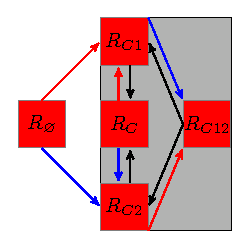
\includegraphics[width=0.3\linewidth]{graphs/article1/figure_7.eps}
\end{center}
\caption{ An history based model for drifting co-circulating
    cross-reactive antigenic clusters. The viruses are supposed to
  contain two antigens: a conserved antigen, shared by strains of the
  resident and the mutant antigenic cluster and a specific antigen,
  specifying each cluster. Naive hosts acquire immunity to both
  conserved and specific part ($R_{Ci}$) resulting in full protection
  toward strains of cluster $i$. Within cluster antigenic drift
  affects only the specific antigen resulting in $R_{Ci} \to R_C$
  transitions at a rate governed by parameter $\gamma$. The shared
  conserved antigen confers partial protection reducing the
  probability of reinfection by a factor $1-\sigma$. Red (blue) arrows
  represent infection by cluster 1 (2). Black arrows represent within
  cluster antigenic evolution. A full description of the assumptions
  leading to this model is provided in section 4 of Supporting
  Information~S1. These hypotheses also enable to recover the model of
  \cite{Goekaydin2007} and therefore render the two frameworks ($SIRI$
  and $SIRS$ within cluster antigenic drift description) readily
  comparable.}
  \label{fig:model_sirs}
\end{figure}



\begin{figure}[!htbp]
\begin{center}
  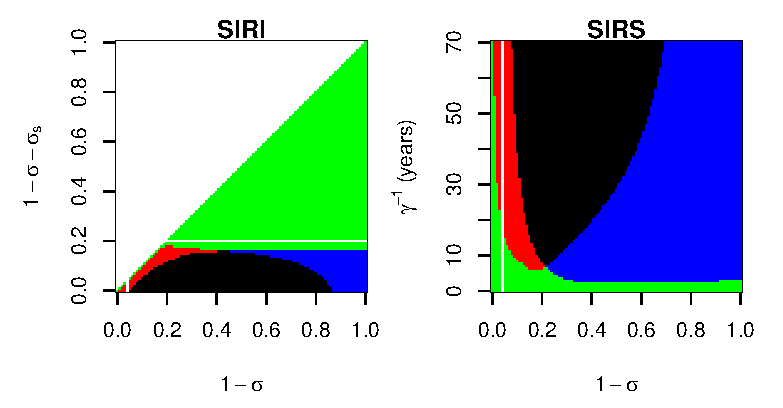
\includegraphics[width=0.7\linewidth]{graphs/article1/figure_8.eps}
\end{center}
  \caption{ Effect of the introduction of within cluster gradual
    antigenic drift on the outcome of the invasion of a new antigenic
    cluster. Comparison of the $SIRS$ model (right) described in
    figure~\ref{fig:model_sirs} and Supporting Information~S1 with the
    $SIRI$ model of \cite{Goekaydin2007} (left). x-axis scale the
    amount of immune escape achieved by the mutant antigenic cluster.
    y-axis represent a measure of within cluster antigenic drift (see
    Supporting Information~S1 for details). Colours: both antigenic
    clusters go extinct (black), the resident cluster only goes
    extinct (successful replacement, red); the mutant cluster only
    goes extinct (blue); no cluster goes extinct (coexistence, green).
    Extinction threshold is set at $N=10^{-7}$. Parameter values are
    given in Table \ref{tab:param} (theoretical set). The horizontal
    white lines of the left graphs situates the reinfections
    thresholds of the $SIRI$ models
    ($1-\sigma-\sigma_s=\frac{1}{R_0}$). The vertical white lines set
    the highest immune escape intensity ($1-\sigma$) for which the
    same model without within cluster antigenic drift predicts
    replacements.}
\label{fig:within_drift}
\end{figure}


Introducing gradual antigenic drift in a minimal model for influenza
also allows to reduce the high critical community size needed to
ensure the persistence of a resident antigenic cluster. A small rate
of gradual antigenic drift have a dramatic effect on the CCS of a
resident antigenic cluster reducing the CCS from 10 millions to 1-2
millions (Supporting Information~S1). CCS closer to one million
renders stochastic effect (such as noise induced temporal asynchrony
\citep{Kamo2002}) important to consider as they could potentially
facilitate coexistence.

These theoretical results corroborate \citet{Finkenstaedt2005},
\citet{Shih2007} and \citet{Suzuki2008} analysis of antigenic drift at
the population level.  \citet{Finkenstaedt2005} have estimated
baseline antigenic drift rate from influenza like illness data using a
model allowing sudden discrete changes and have shown that it was
significantly different from zero. \citet{Shih2007}, using a method
with a higher power of detection of positive selection than previous
studies, have shown that within antigenic cluster change could be more
important than traditionally (\textit{e.g} \citet{Wolf2006}) believed.

Gradual antigenic drift should thus be part of a minimal model for
influenza A along with punctuated immune escape.

%\clearpage

\subsubsection{Functional constraints}

Functional constraints are well established for influenza A
\citep{Rambaut2008, Gog2008, Du2008}. For instance, it has been
established that cooperative activities of both HA and NA are critical
for influenza virus infection and release \citep{Wagner2002}.
Functional constraints can induce a fitness cost associated to an
antigenic escape mutation. Lower fitness of the mutant cluster could
be beneficial for the replacement dynamics as by decreasing the
strength of the initial invasion, functional constraints could also
decrease the risk of epidemic fadeout and long refractory periods that
follow high depletion of susceptibles. %
A simple way to handle functional constraints is to consider a
relation between the mutant cluster transmission rates ($\beta_{mut}$)
and its ability to escape previous immunity (governed by $\sigma$).
Without loss of generality, functional constraint can be introduced by
lowering $\beta_{mut}$ (assuming $\beta_{mut}=\alpha \beta_{res}$ with
$\frac{1}{R_0^{res}} \leq \alpha \leq 1$) to ensure that $1 \leq
R_0^{mut} \leq R_0^{res}$. Using section~Results results we can
calculate the threshold value of $\sigma$, equal to $\sigma^*$,
necessary for the antigenic cluster invasion. In case of both $HB$ and
$SBRS$ models, the threshold is defined by $\sigma < \frac{\alpha
  R_0^{res}-1}{\alpha (R_0^{res} -1)}$. Functional constraints can
explain why immune escape mutations do not generate unrealistic high
epidemics (Supporting Information~S1). To compare our results to
\citet{Koelle2006} model, we have neglected such constraint but they
should be considered in further investigations. Such inclusion would
need to incorporate compensatory mutations \citep{Du2008} to restore
original function and re-increase the impaired $\beta_{mut}$.
\\

\subsubsection{Multiple infections before acquiring immunity}

As we have shown through simulations (figures~\ref{fig:deter},
\ref{fig:reinv_theo12} and \ref{fig:replace}), subtype replacement (as
a consequence of antigenic shifts) appears impossible except in the
case of the questionable $SBRI$ model. This is contrary to what have
been observed during previous 1957's Asian flu and 1968's Hong Kong
flu pandemics \citep{Earn2000}. This lack of realism was reported by
\citet{Ferguson2003} in case of history based models and had been
partially solved by including temporary cross-immunity
\citep{Webster1992}. However, other proposals that temporary
cross-immunity could also be relevant. For instance, by using data of
the first introduction of H3N2 type A influenza on the island of
Tristan da Cunha in 1971, \citet{Mathews2007} show that two epidemics
separated by 20 days only have affected the population and most of the
hosts have been infected twice. This is different from the
conventional knowledge of influenza immunology and suggests that
multiple infection could be necessary before developing long term
immunity. This creates far more susceptible individuals than expected
from our models and greatly favours the persistence of the new
subtype. It remains to be tested whether the persistence of the new
subtype is sufficient to drive the resident subtype to extinction.
Concerning epidemic influenza, the need to incorporate multiple
infection before the acquisition of immunity deserves further
attention.
\\

\vspace{1cm}

As a last point, \citet{Recker2007} have reopened a theory on
influenza antigenic evolution dominant in 1960 \citep{Francis1960}.
Within this theory, the virus population is characterised by a limited
set of antigenic types, all of which may be continuously
(re-)generated from preexisting strains. \citet{Recker2007} have shown
that sampling from a population where a limited set of antigenic types
describe complex dynamics can reproduce the specific patterns of
antigenic cluster succession revealed by \citet{Smith2004} analysis.
This view offers an alternative explanation to the sequential
antigenic drift scenario examined in this paper. Recent data, analysed
by phylogenetic and coalescent based approaches, strongly suggest that
influenza A dynamics is part of a source-sink system where the source
could be a reservoir of a limited set of antigenic types
\citep{Alonso2007a, Nelson2007b, Holmes2005, Nelson2006, Viboud2006,
  Rambaut2008, Russell2008}. However, it remains to be seen to what
extent restriction of viral genetic diversity could be achieved by
\citet{Recker2007} model. This model strongly depends on antigenic
recycling to justify the low dimensionality of the phenotype space,
but antigenic recycling does not seem to be supported by current data
\citep{Minayev2008, Minayev2009}.\\

\vspace{1cm}


In conclusion, our findings finally suggest the importance of gradual
antigenic drift for epidemic dynamics even in the presence of
punctuated immune escape. Our results indicate that status based model
with reduced infectivity assumption can have profound consequences on
the transient dynamics of strains invasion. In case of influenza, this
model should be used with caution as it includes biologically
unsupported processes that can induce serious bias.


% Do NOT remove this, even if you are not including acknowledgments
\section{Acknowledgments}

The authors are grateful to Mercedes Pascual for helpful discussions.




%%% Local Variables: 
%%% mode: latex
%%% TeX-master: "../../phD"
%%% End: 
